% include the figures path relative to the master file
%\graphicspath{ {./content/method/figures/} }

\section{Related work}\label{sec:rw}


\begin{figure*}
\begin{center}
   \subfigure[Vitreomacular traction.]{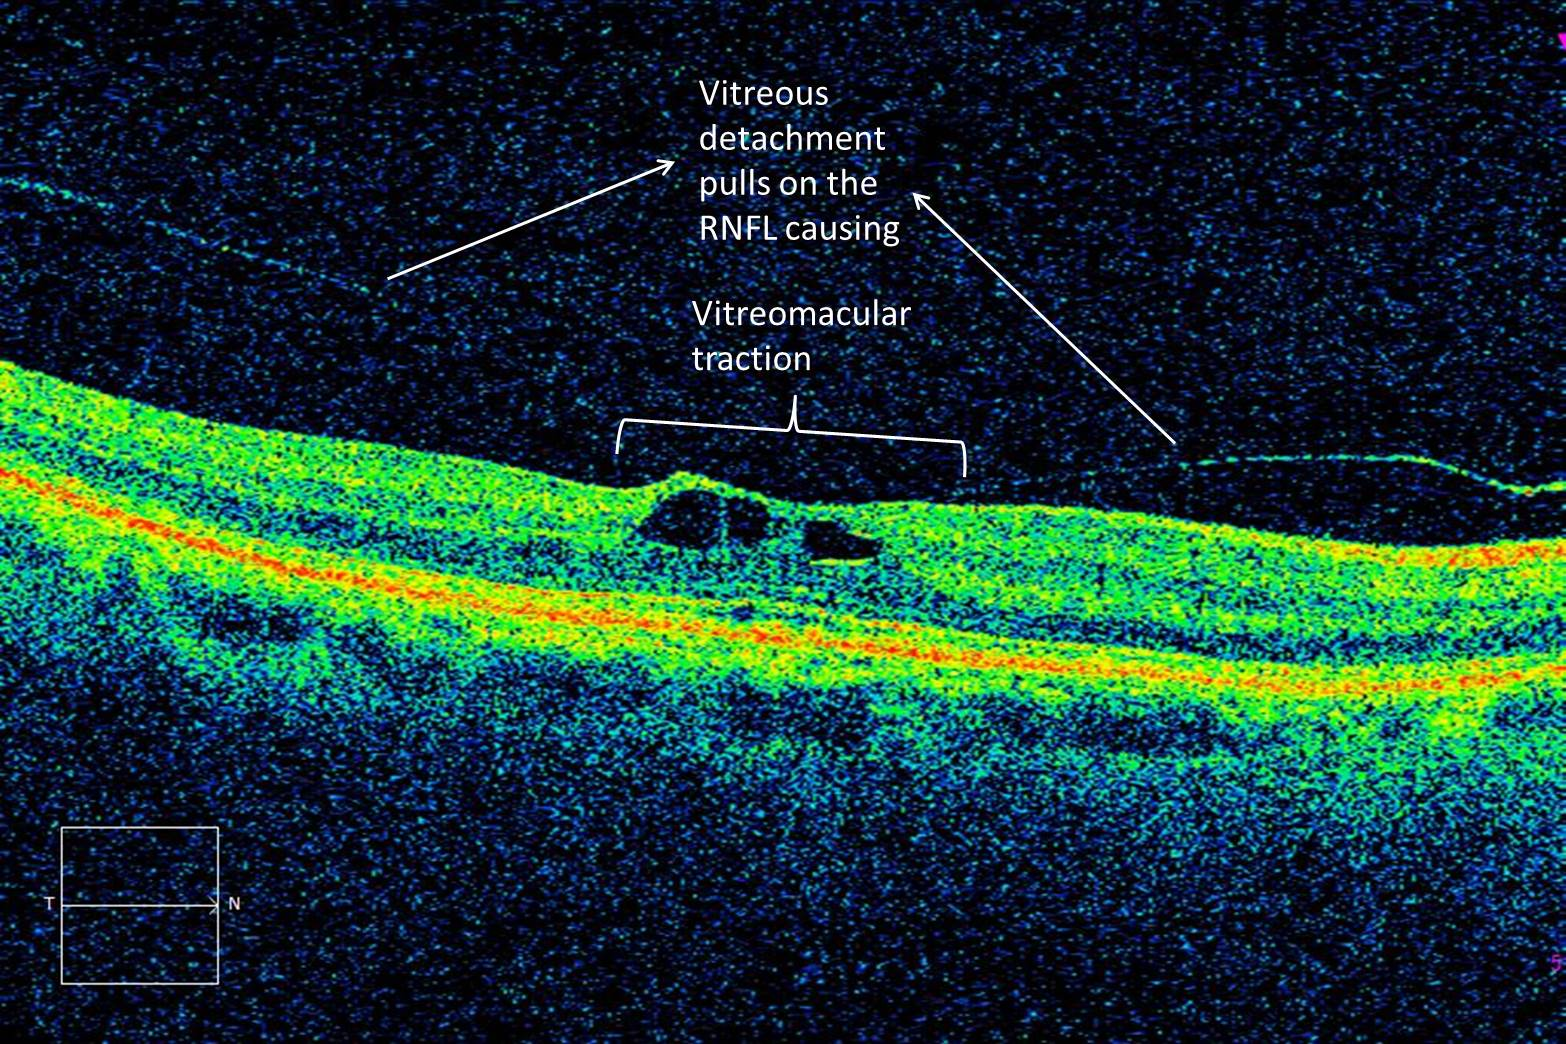
\includegraphics[width=0.3\textwidth, height = 0.15\textheight]{./content/method/figures/Vitreomacular}}\
   \subfigure[Rethinal thickening.]{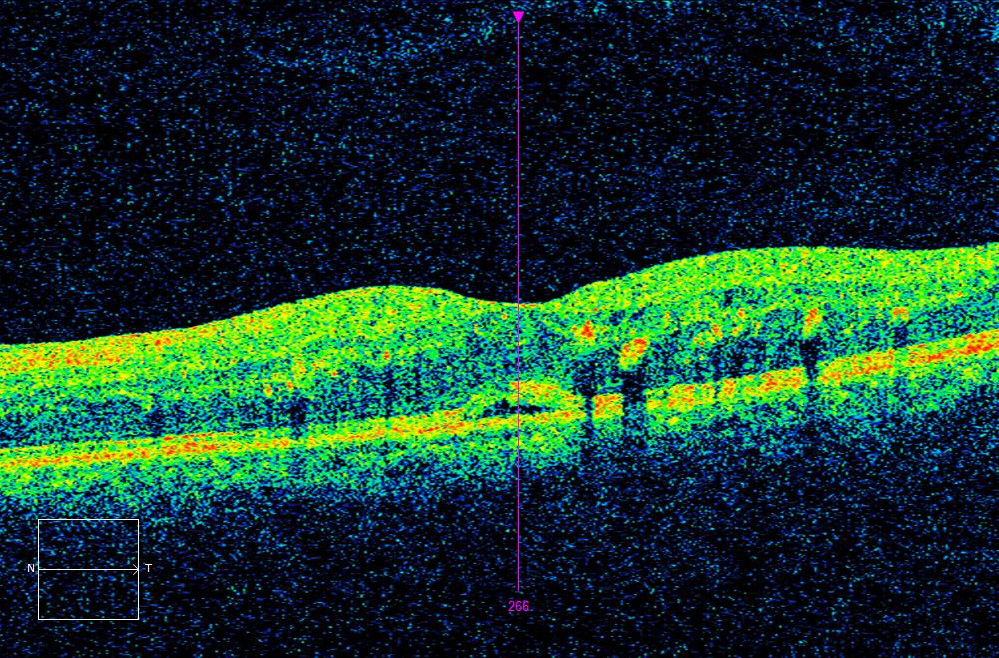
\includegraphics[width = 0.3\textwidth,height = 0.15\textheight]{./content/method/figures/RE}} \
   \subfigure[Cyst spaces, causing central and parafoveal retina thickening.]{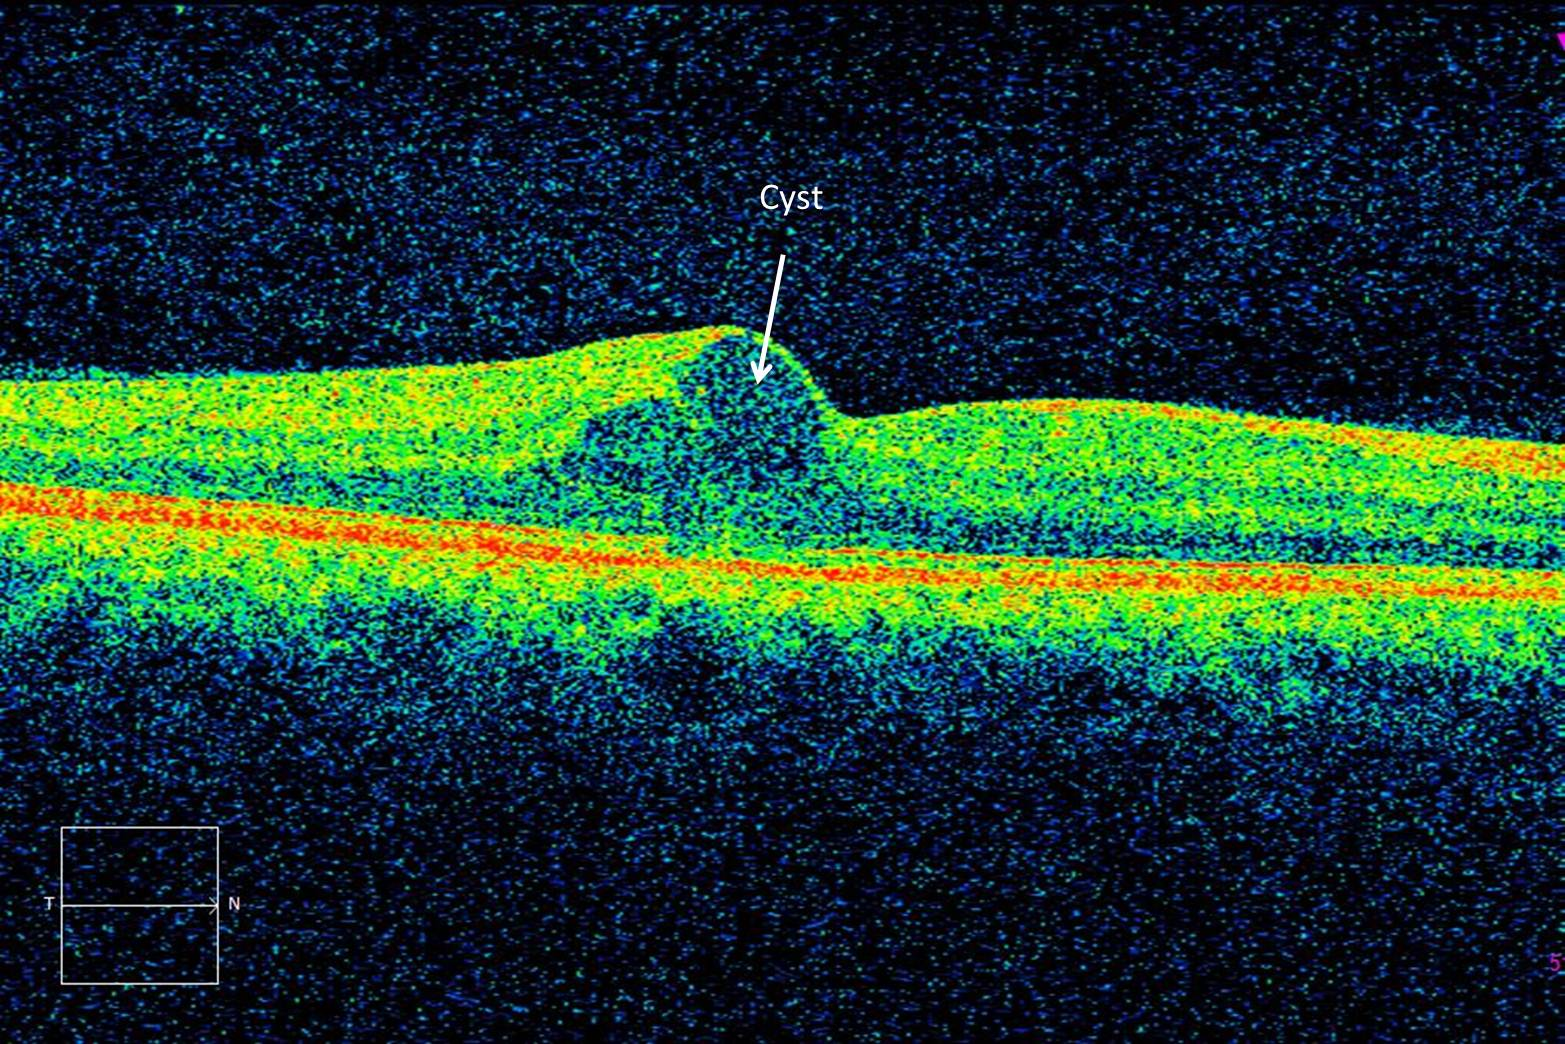
\includegraphics[width=0.3\textwidth,height = 0.15\textheight]{./content/method/figures/Cyst}}\\
   \subfigure[Cyst spaces and hard exudates, causing central retinal thickening.]{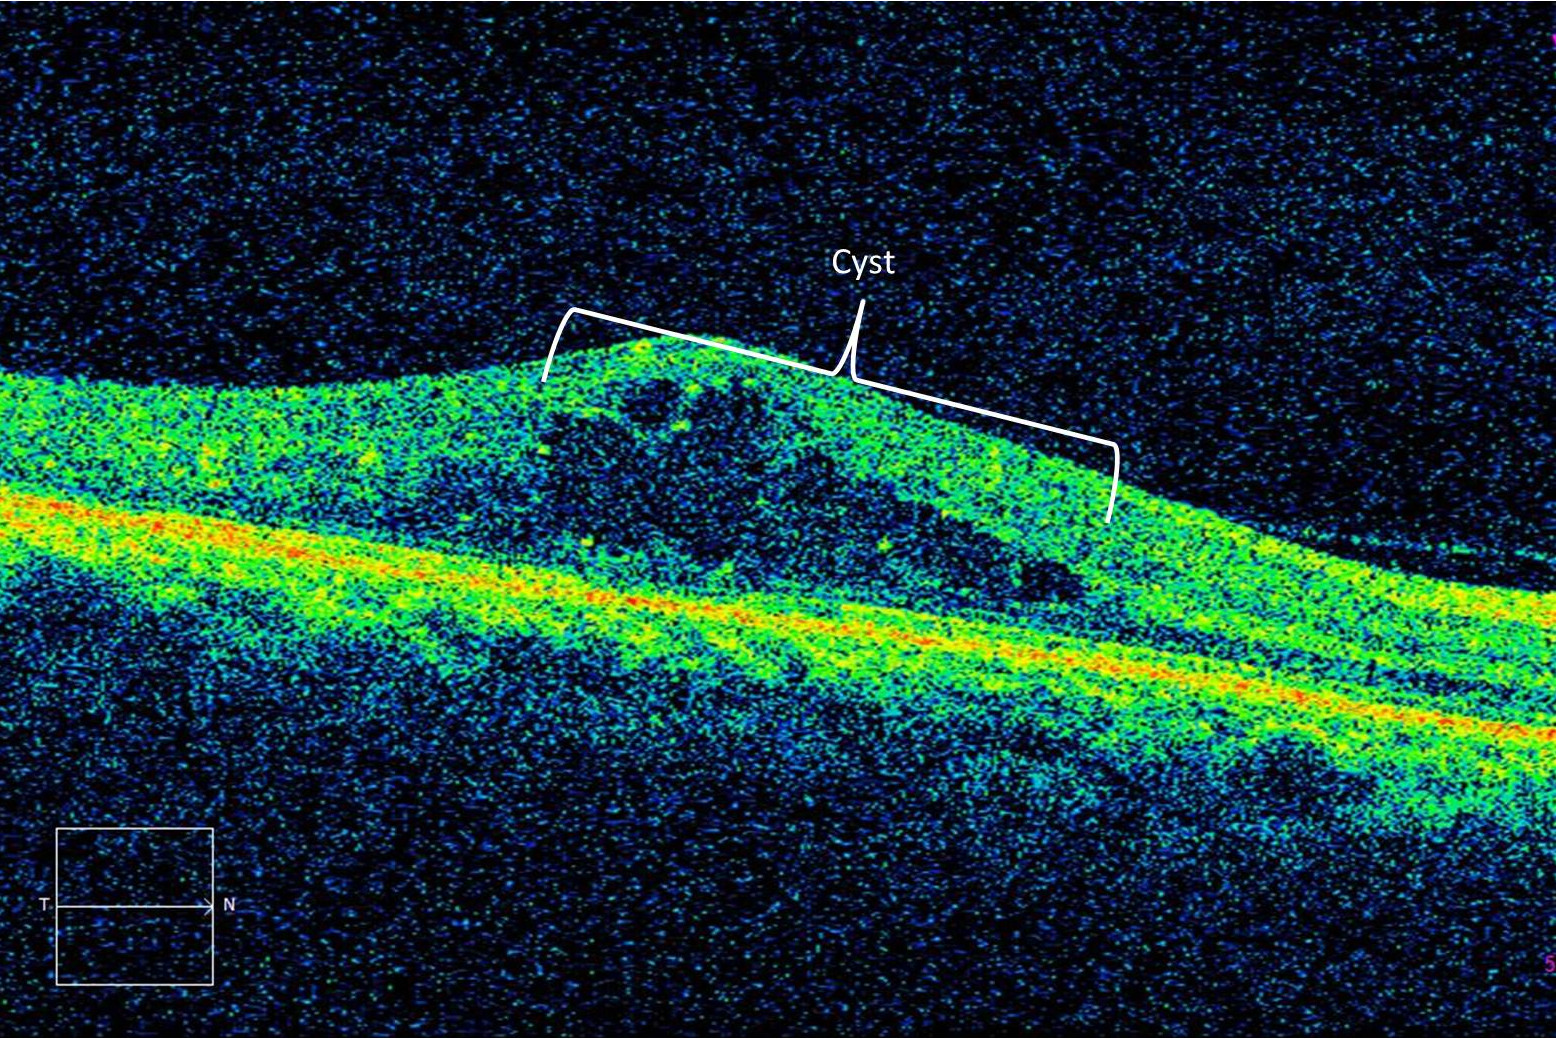
\includegraphics[width = 0.3\textwidth,height = 0.15\textheight]{./content/method/figures/Cyst+HE+RE}} \
   \subfigure[CSR (subretinal fluid), causing central and parafoveal thickening.]{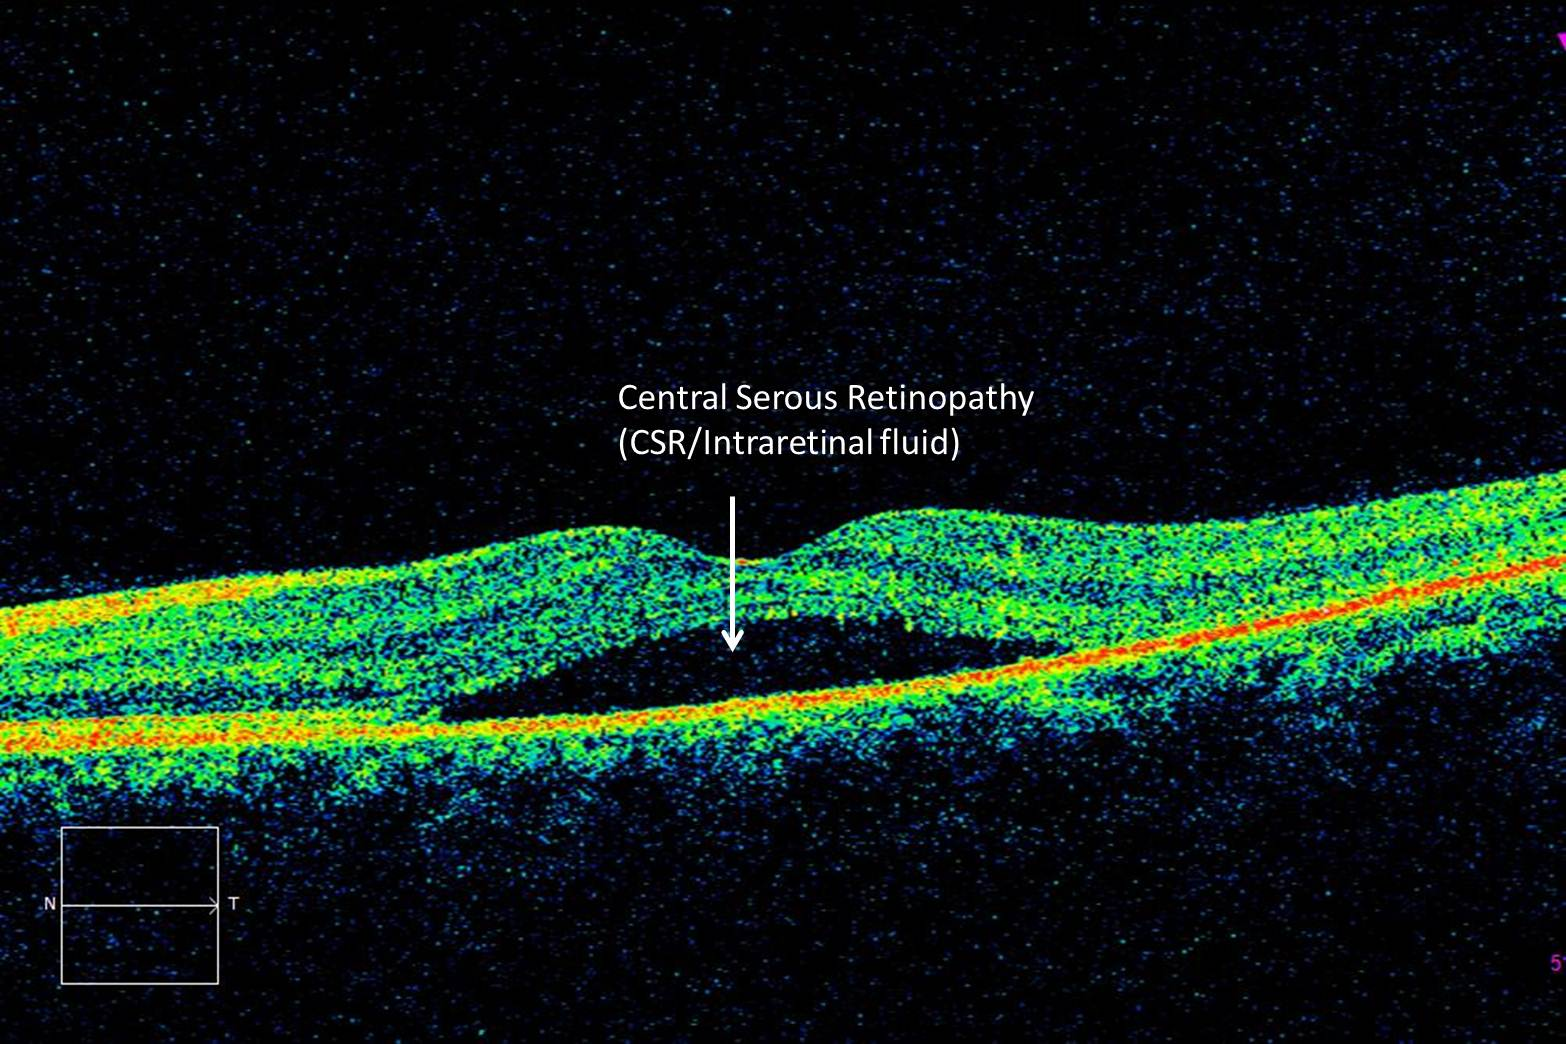
\includegraphics[width = 0.3\textwidth,height = 0.15\textheight]{./content/method/figures/CSR}} \
   \subfigure[CSR, hard exudates and cyst spaces.]{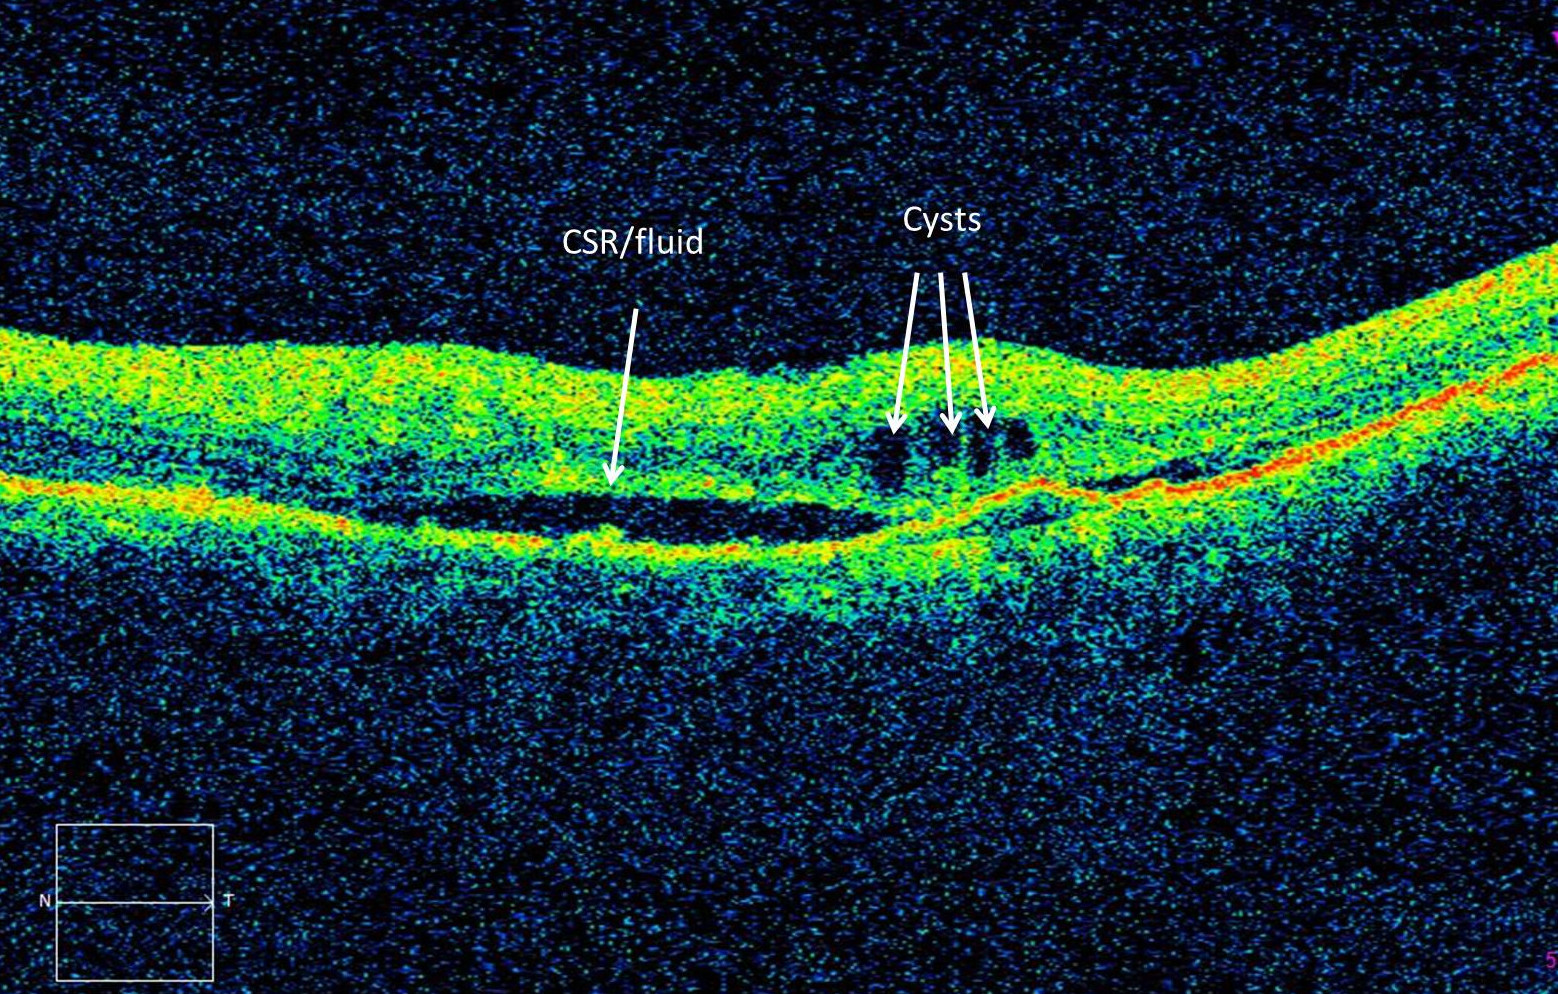
\includegraphics[width = 0.3\textwidth,height = 0.15\textheight]{./content/method/figures/Cyst+CSR+HE}} \\
   \subfigure[Cyst spaces, causing retinal thickening.]{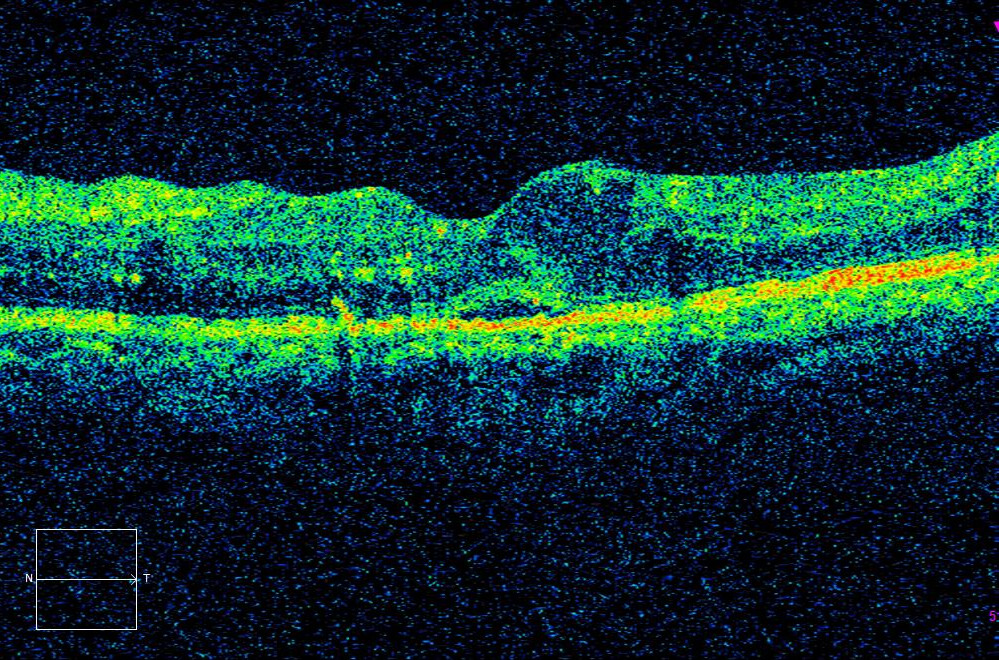
\includegraphics[width = 0.3\textwidth,height = 0.15\textheight]{./content/method/figures/Cyst+RE}} \
   \subfigure[CSR and hard exudates, causing retinal thickening.]{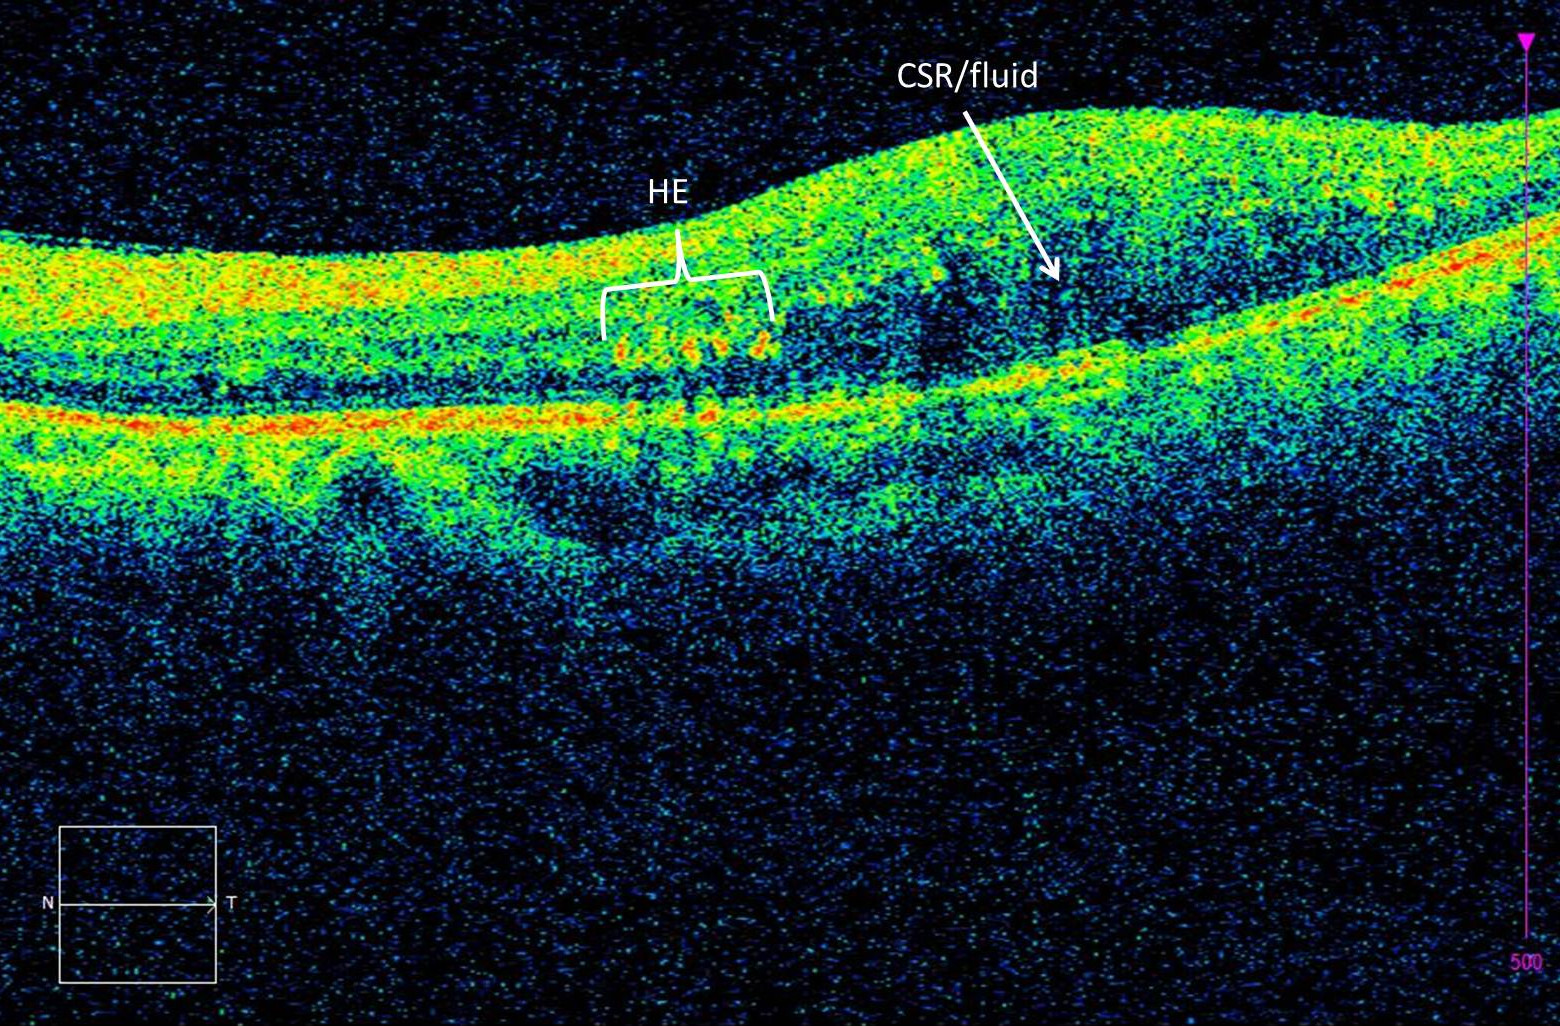
\includegraphics[width = 0.3\textwidth,height = 0.15\textheight]{./content/method/figures/CSR+HE+RE}} \   
   \subfigure[Cyst spaces causing parafoveal thickening.]{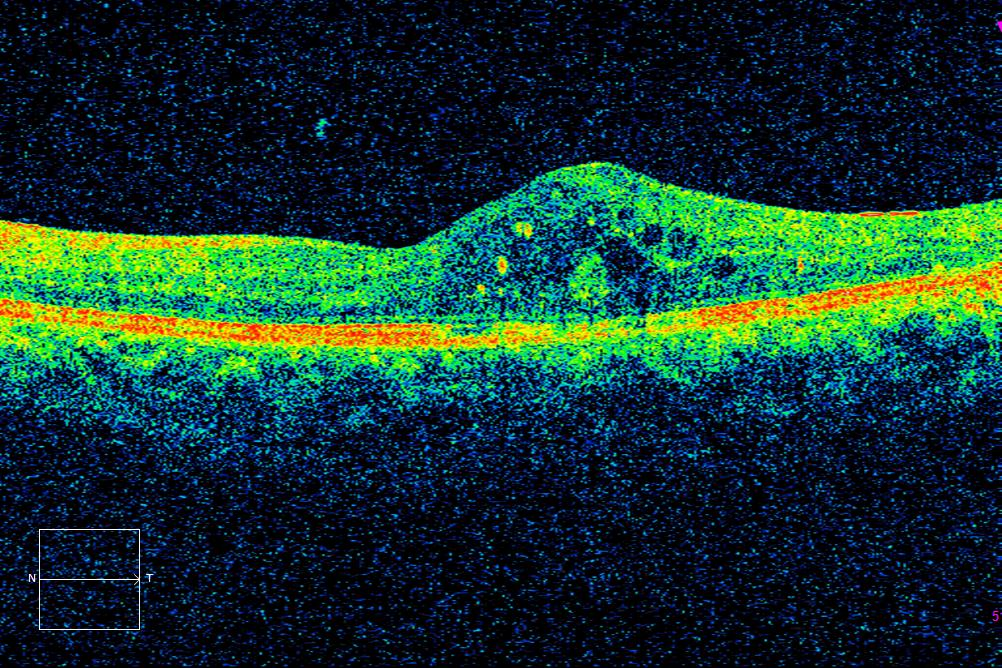
\includegraphics[width = 0.3\textwidth,height = 0.15\textheight]{./content/method/figures/Cyst+RE_parafovel}} \\
    
\end{center}
    \caption{Examples of \gls{dme} cases in \gls{seri} dataset.}
  \label{fig:bbdd}
\end{figure*}


\begin{figure*}
\centering
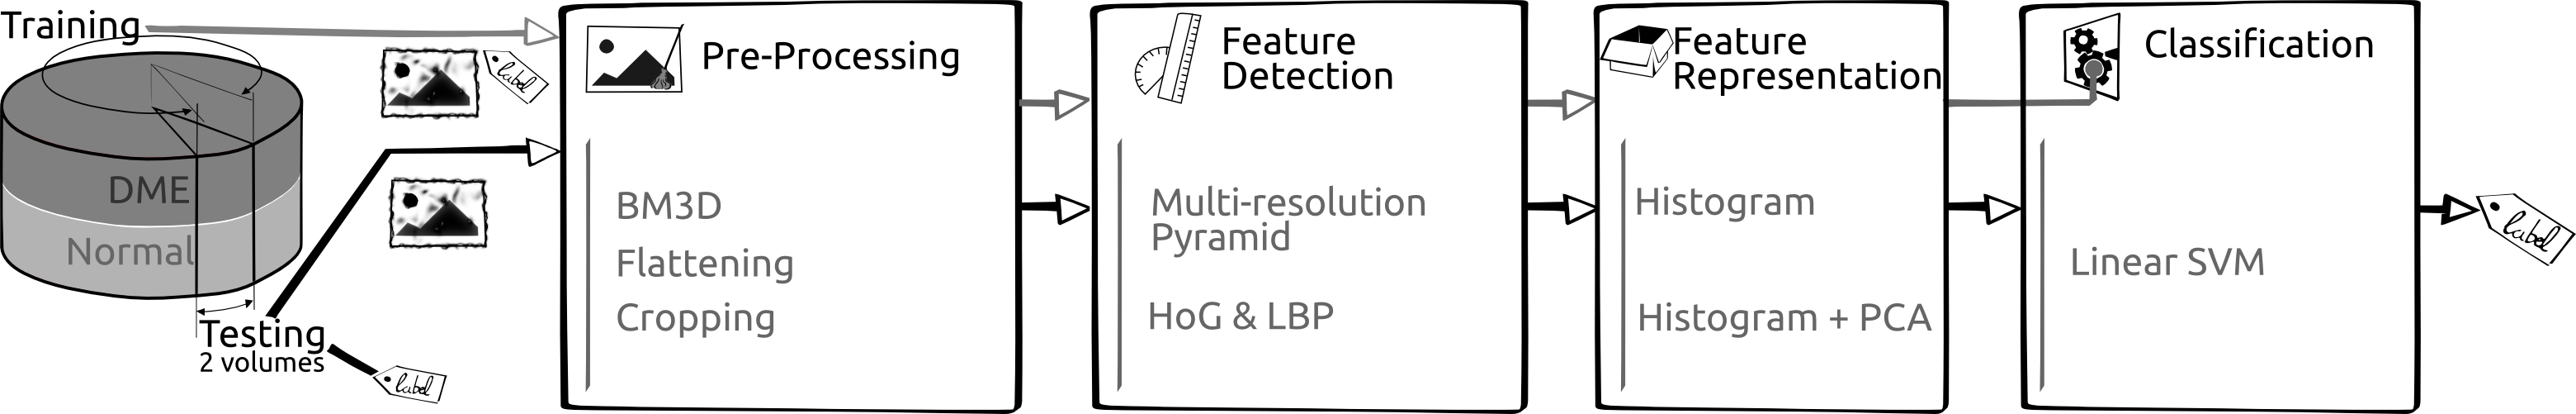
\includegraphics[width = 0.98\textwidth]{./content/method/figures/khaled_embc}
\caption{Proposed classification pipeline.}
\label{fig:fig3}
\end{figure*}

Srinivasan~\textit{et al.} proposed a classification method to distinguish normal \gls{oct} volumes from \gls{dme} and \gls{amd} volumes \cite{srinivasan2014fully}.
The \gls{oct} images are pre-processed by reducing the speckle noise by enhancing the sparsity in a transform-domain and flattening the retinal curvature to reduce the inter-patient variations.
Then, \gls{hog} are extracted for each slice of a volume and fed to a linear \gls{svm}.
This method was applied onto a dataset of 45 patients equally subdivided into the three aforementioned classes and led to a correct classification rate of 100\%, 100\% and 86.67\% for normal, \gls{dme} and \gls{amd} patients, respectively.
The images that were used in their paper, are publically available but are already preprocessed (noise removed), do not offer a huge variability in term of \gls{dme} lesions, have different sizes for the \gls{oct} volumes, and some of them (without specifying which) have been excluded for the training phase; all these reasons prevent us from using this dataset to benchmark our work.
Venhuizen~\textit{et al.} recently proposed a method for \gls{oct} images classification using the \gls{bow} models \cite{Sivic2003}.
The method starts with the detection and selection of keypoints in each individual B-scan, by keeping the most salient points corresponding to the top 3\% of the vertical gradient values.
Then, a 9~$\times$~9 pixels texton is extracted around each keypoint, and \gls{pca} is applied to reduce the dimension of every texton from 81 to 9. 
All extracted feature vectors are used to create a dictionnary using k-means clustering.
Then, each \gls{oct} volume is represented as an histogram that captures the codeword occurrences.
These histograms are used as feature vector to train a \gls{rf} classifier with a maximum of 100 trees.
The method was used to classify \gls{oct} volumes between \gls{amd} and normal cases and achieved an \gls{auc} of 0.984 with a dataset of 384 \gls{oct} volumes \cite{venhuizen2015automated}.
Liu~\textit{et al.} proposed a methodology for detecting macular pathology in \gls{oct} images using \gls{lbp} and gradient information as attributes \cite{liu2011automated}.
The method starts by aligning and flattening the images and creating a 3-level multi-scale spatial pyramid.
The edge and \gls{lbp} histograms are then extracted from each 80 block of every level of the pyramid.
All the obtained histograms are concatenated into a global descriptor whose dimensions are reduced using \gls{pca}.
Finally a \gls{svm} with an \gls{rbf} kernel is used as classifier.
The method achieved good results in detection \gls{oct} scan containing different pathology such as \gls{dme} or \gls{amd}, with an \gls{auc} of 0.93 using a dataset of 326 \gls{oct} scans.
%In this paper we propose an automatic framework for identification of DME patients versus normal subjects using OCT volumes.
Lema\^{i}tre~\textit{et al.} developed a classification framework  based on \gls{lbp} features to describe the texture of \gls{oct} images and dictionary learning using the \gls{bow} models \cite{lemaitre2015}.
They proposed to extract 2D and 3D \gls{lbp} features from \gls{oct} images and volumes, respectively.
The \gls{lbp} descriptors are either extracted from the entire sample or local patches within individual samples.
Numerous experiments were conducted and the authors achieved a sensitivity and specificity of 81.2\% and 93.2\% for their best configuration.
On the same dataset, a different approach which consists in  addressing this issue as an anomaly detection problem was recently proposed by Sankar~\textit{et al.} \cite{sankar2016}.
In their method, the authors propose a technique that not only allow the classification of the \gls{oct} volume, but also enables the identification of the individual diseased B-scans inside the volume.
This approach is based on modeling the appearance of normal \gls{oct} images with a \gls{gmm} and detecting abnormal \gls{oct} images as outliers.
The classification of an \gls{oct} volume is based on the number of detected outliers.
Experimental results with two different datasets show that the proposed method achieves a sensitivity and a specificity of 80\% and 93\% on the first dataset, and 100\% and 80\% on the second one.
The proposed method achieves better classification performance than other recently published work but it requires to tune the \gls{gmm} parameters and it should be tested on a larger database.





